\chapter{Nucleótidos y ácidos nucleicos}\label{ch:b1:nucleic-acids}

Viértase etanol frío sobre una disolución de \omterm{def:b1:cell-unit-of-life:cell}{células} rotas y aparecerá una
nube blanca de fibras que puede enrollarse en una varilla de vidrio: es el
\omterm{def:b1:nucleic-acids:chain}{ADN}, la molécula que lleva todas las instrucciones del \omterm{def:b1:organism-environment:organism}{organismo}, visible a
simple vista. Dos metros de él están plegados en cada núcleo humano; está
escrito por entero en un alfabeto de cuatro letras, se lee en un solo
sentido y se copia separando dos hebras que encajan la una en la otra como
una mano y su guante. Este capítulo describe los \omterm{def:b1:nucleic-acids:nucleotide}{nucleótidos} --- letras,
\omterm{def:b1:water-small-molecules:atp}{moneda energética} y coenzimas a la vez ---, las cadenas que forman, la \omterm{thm:b1:nucleic-acids:helix}{doble
hélice} y las pruebas que la sostienen, lo que ocurre cuando se funde y se
vuelve a aparear, y los \omterm{def:b1:nucleic-acids:chain}{ARN} que llevan su mensaje al resto de la \omterm{def:b1:cell-unit-of-life:cell}{célula}.

\section{Nucleótidos}

\begin{definition}[Nucleótido]\label{def:b1:nucleic-acids:nucleotide}
Un \emph{nucleótido}\index{nucleótido} consta de tres partes: una
\emph{base}\index{base nitrogenada} nitrogenada --- una
\emph{purina}\index{purina} (adenina A, guanina G: dos anillos condensados)
o una \emph{pirimidina}\index{pirimidina} (citosina C, timina T, uracilo U:
un anillo) ---; un azúcar de cinco carbonos, la \emph{ribosa} en el \omterm{def:b1:nucleic-acids:chain}{ARN} o la
\emph{2$'$-desoxirribosa} en el \omterm{def:b1:nucleic-acids:chain}{ADN} (que carece del hidroxilo del carbono
$2'$); y de uno a tres grupos \emph{fosfato} sobre el carbono $5'$ del
azúcar. La base se une al carbono $1'$; los carbonos del azúcar se numeran
con prima para distinguirlos de los de la base. La base más el azúcar forman
un \emph{nucleósido} (adenosina, guanosina, citidina, timidina, uridina);
con los fosfatos es un nucleótido (AMP, ADP, \omterm{def:b1:water-small-molecules:atp}{ATP} y sus parientes).
\end{definition}

\begin{omfigure}
\begin{tikzpicture}[font=\footnotesize, line cap=round, line join=round]
  % phosphates
  \foreach \i/\c in {0/omThm!15,1/omThm!25,2/omThm!35} {
    \draw[thick, omThm!80!black, fill=\c, rounded corners=3pt] (1.3*\i,0.9) rectangle (1.3*\i+1.1,1.9);
    \node at (1.3*\i+0.55,1.4) {$\mathrm{P}$};
  }
  \node[anchor=south, align=center] at (1.65,2.15) {fosfatos: $\gamma$, $\beta$, $\alpha$\\ (enlaces anhídrido entre ellos)};
  \draw[thick] (3.3,1.4) -- (4.0,1.4);
  % sugar pentagon
  \draw[thick, omDef!80!black, fill=omDef!15] (4.0,1.4) -- (4.55,2.05) -- (5.45,2.05) -- (6.0,1.4) -- (5.0,0.85) -- cycle;
  \node at (5.0,1.5) {ribosa};
  \node[font=\scriptsize] at (3.85,1.15) {$5'$};
  \node[font=\scriptsize] at (4.55,2.25) {$4'$};
  \node[font=\scriptsize] at (5.45,2.25) {$1'$};
  \node[font=\scriptsize] at (6.15,1.15) {$2'$};
  \node[font=\scriptsize] at (5.0,0.6) {$3'$};
  \draw[thick] (5.0,0.85) -- (5.0,0.2) node[below] {OH};
  \draw[thick] (6.0,1.4) -- (6.6,1.0) node[right] {OH (H en la desoxirribosa)};
  % base
  \draw[thick] (5.45,2.05) -- (5.9,2.7);
  \draw[thick, omExo!80!black, fill=omExo!15, rounded corners=3pt] (5.4,2.7) rectangle (7.6,3.7);
  \node at (6.5,3.2) {base (A, G, C, U/T)};
  \node[anchor=west, align=left, gray] at (8.2,3.0) {nucleósido = base + azúcar\\ nucleótido = nucleósido + fosfato(s)\\ ATP = adenina + ribosa + tres fosfatos};
\end{tikzpicture}

{\small Las partes de un \omterm{def:b1:nucleic-acids:nucleotide}{nucleótido}: una \omterm{def:b1:nucleic-acids:nucleotide}{base} sobre el carbono $1'$ de una
pentosa y fosfatos sobre el carbono $5'$. El hidroxilo del $3'$ es donde se
unirá el \omterm{def:b1:nucleic-acids:nucleotide}{nucleótido} siguiente de la cadena; la posición $2'$ distingue el
\omterm{def:b1:nucleic-acids:chain}{ARN} (OH) del \omterm{def:b1:nucleic-acids:chain}{ADN} (H).}
\end{omfigure}

\begin{proposition}[Los nucleótidos desempeñan tres tareas]\label{prop:b1:nucleic-acids:threejobs}
Además de ser los monómeros del \omterm{def:b1:nucleic-acids:chain}{ADN} y del \omterm{def:b1:nucleic-acids:chain}{ARN}, los \omterm{def:b1:nucleic-acids:nucleotide}{nucleótidos} son la
\emph{\omterm{def:b1:water-small-molecules:atp}{moneda energética}} de la \omterm{def:b1:cell-unit-of-life:cell}{célula} --- \omterm{def:b1:water-small-molecules:atp}{ATP} y GTP, cuyos \omterm{def:b1:water-small-molecules:atp}{enlaces
fosfoanhídrido} (\cref{ch:b1:water-small-molecules}) pagan la síntesis, el
transporte y el movimiento ---; sus \emph{coenzimas} --- $\mathrm{NAD^+}$,
$\mathrm{NADP^+}$ y FAD, que transportan electrones en la respiración y en
la fotosíntesis (\cref{ch:b1:respiration-fermentation}), y la coenzima A,
que transporta grupos acilo ---; y sus \emph{mensajeros} --- el AMP cíclico,
que retransmite señales hormonales dentro de las \omterm{def:b1:cell-unit-of-life:cell}{células}. Todos ellos son
\omterm{def:b1:nucleic-acids:nucleotide}{nucleótidos} de adenina o están construidos sobre ellos: la misma molécula
que deletrea el mensaje alimenta su ejecución.
\end{proposition}

\section{La cadena polinucleotídica}

\begin{definition}[Enlace fosfodiéster, polaridad]\label{def:b1:nucleic-acids:chain}
Los \omterm{def:b1:nucleic-acids:nucleotide}{nucleótidos} se unen en un
\emph{polinucleótido}\index{polinucleótido} mediante \emph{enlaces
fosfodiéster}\index{enlace fosfodiéster}: el fosfato del carbono $5'$ de un
\omterm{def:b1:nucleic-acids:nucleotide}{nucleótido} se enlaza al hidroxilo $3'$ del siguiente. La cadena tiene por
tanto un \emph{esqueleto} de azúcar y fosfato, uniforme y cargado
negativamente (una carga por fosfato), del que las \omterm{def:b1:nucleic-acids:nucleotide}{bases} sobresalen como una
secuencia; y tiene un sentido: un \emph{extremo $5'$}\index{5' end@extremo $5'$} con un fosfato libre y un
\emph{extremo $3'$}\index{3' end@extremo $3'$} con un hidroxilo libre. Las
secuencias se escriben y se leen de $5' \to 3'$, el sentido en que se
sintetizan las cadenas. El \emph{ADN}\index{ADN} (ácido desoxirribonucleico)
usa desoxirribosa y las \omterm{def:b1:nucleic-acids:nucleotide}{bases} A, G, C, T; el \emph{ARN}\index{ARN} (ácido
ribonucleico) usa ribosa y A, G, C, U.
\end{definition}

\begin{omfigure}
\begin{tikzpicture}[font=\footnotesize, line cap=round]
  \foreach \i/\b in {0/A,1/C,2/G,3/T} {
    \draw[thick, omThm!80!black, fill=omThm!25, rounded corners=2pt] (0.3,-1.6*\i+0.15) rectangle (0.9,-1.6*\i+0.75);
    \node at (0.6,-1.6*\i+0.45) {P};
    \draw[thick, omDef!80!black, fill=omDef!15] (1.3,-1.6*\i-0.1) -- (1.6,-1.6*\i+0.3) -- (2.2,-1.6*\i+0.3) -- (2.5,-1.6*\i-0.1) -- (1.9,-1.6*\i-0.5) -- cycle;
    \node[font=\scriptsize] at (1.9,-1.6*\i-0.1) {azúcar};
    \draw[thick] (0.9,-1.6*\i+0.45) -- (1.3,-1.6*\i-0.1);
    \node[font=\scriptsize] at (1.2,-1.6*\i+0.4) {$5'$};
    \node[font=\scriptsize] at (2.0,-1.6*\i-0.75) {$3'$};
    \draw[thick] (2.2,-1.6*\i+0.3) -- (2.9,-1.6*\i+0.3);
    \draw[thick, omExo!80!black, fill=omExo!15, rounded corners=2pt] (2.9,-1.6*\i+0.0) rectangle (3.7,-1.6*\i+0.6);
    \node at (3.3,-1.6*\i+0.3) {\b};
  }
  \foreach \i in {0,1,2} { \draw[thick] (1.9,-1.6*\i-0.5) -- (0.6,-1.6*\i-0.85); }
  \node[anchor=east, align=right] at (0.1,0.9) {extremo $5'$:\\ fosfato libre};
  \node[anchor=east, align=right] at (0.1,-5.5) {extremo $3'$:\\ hidroxilo libre};
  \draw[thick] (1.9,-5.3) -- (1.9,-5.7) node[below, font=\scriptsize] {OH};
  \draw[->, very thick, gray] (4.6,0.6) -- (4.6,-5.2) node[midway, right, align=left] {se lee y se escribe\\ de $5' \to 3'$:\\ esta hebra es\\ $5'$-ACGT-$3'$};
  \draw[thick, omThm!80!black] (0.4,-0.9) -- (0.4,-1.3);
  \node[anchor=west, align=left, gray] at (7.4,-2.6) {esqueleto: azúcar y fosfato\\ alternos, una carga negativa\\ por fosfato\\ bases: la parte variable,\\ la secuencia};
\end{tikzpicture}

{\small Una cadena de cuatro \omterm{def:b1:nucleic-acids:nucleotide}{nucleótidos}. El fosfato $5'$ de cada \omterm{def:b1:nucleic-acids:nucleotide}{nucleótido}
se une al hidroxilo $3'$ del que está encima por un \omterm{def:b1:nucleic-acids:chain}{enlace fosfodiéster}; la
cadena va de un extremo $5'$ a un extremo $3'$ y las \omterm{def:b1:nucleic-acids:nucleotide}{bases} cuelgan de un
esqueleto uniforme.}
\end{omfigure}

\begin{example}[El ARN es frágil, el ADN es duradero]\label{ex:b1:nucleic-acids:fragile}
El hidroxilo $2'$ de la ribosa puede atacar al \omterm{def:b1:nucleic-acids:chain}{enlace fosfodiéster} vecino:
en un álcali suave el \omterm{def:b1:nucleic-acids:chain}{ARN} se hidroliza a \omterm{def:b1:nucleic-acids:nucleotide}{nucleótidos} en cuestión de horas,
mientras que el \omterm{def:b1:nucleic-acids:chain}{ADN}, que carece de ese hidroxilo, resiste la ebullición en
álcali y se ha recuperado intacto de huesos de decenas de miles de años. El
uracilo del \omterm{def:b1:nucleic-acids:chain}{ARN} es la timina sin su grupo metilo; el \omterm{def:b1:nucleic-acids:chain}{ADN} usa timina para que
la citosina, que pierde lentamente su grupo amino y se convierte en uracilo,
pueda reconocerse como dañada y repararse: un uracilo en el \omterm{def:b1:nucleic-acids:chain}{ADN} es siempre
un error.
\end{example}

\section{La doble hélice}

\begin{proposition}[Las reglas de Chargaff]\label{prop:b1:nucleic-acids:chargaff}
\index{reglas de Chargaff}
En el \omterm{def:b1:nucleic-acids:chain}{ADN} de cualquier \omterm{def:b1:organism-environment:organism}{organismo} la cantidad de adenina iguala a la de
timina y la de guanina a la de citosina ($A = T$, $G = C$, y por tanto
\omterm{def:b1:nucleic-acids:nucleotide}{purinas} $=$ \omterm{def:b1:nucleic-acids:nucleotide}{pirimidinas}), mientras que el cociente $(G + C)/(A + T)$ varía
de una especie a otra (del \qty{25}{\%} al \qty{75}{\%} de $G + C$).
\end{proposition}
\begin{proof}[Evidencia]
\omterm{prop:b1:nucleic-acids:chargaff}{Chargaff} (1950) hidrolizó \omterm{def:b1:nucleic-acids:chain}{ADN} de muchos \omterm{def:b1:organism-environment:organism}{organismos} y separó las \omterm{def:b1:nucleic-acids:nucleotide}{bases} por
cromatografía, midiendo cada una por su absorción ultravioleta. Las
igualdades se cumplieron dentro del error experimental para todos los \omterm{def:b1:nucleic-acids:chain}{ADN};
el contenido en $G + C$ no, y era el mismo en todos los \omterm{def:b1:body-plans-tissues:tissue}{tejidos} de un mismo
\omterm{def:b1:organism-environment:organism}{organismo}.
\end{proof}

\begin{theorem}[La doble hélice de Watson y Crick]\label{thm:b1:nucleic-acids:helix}
\index{doble hélice}\index{par de bases}\index{antiparalelo}
El \omterm{def:b1:nucleic-acids:chain}{ADN} son dos cadenas polinucleotídicas enrolladas en torno a un eje común
formando una \emph{\omterm{thm:b1:nucleic-acids:helix}{doble hélice}} dextrógira: los esqueletos de azúcar y
fosfato por fuera y las \omterm{def:b1:nucleic-acids:nucleotide}{bases} dentro, planas y apiladas perpendicularmente
al eje. Las cadenas son \emph{antiparalelas} (una va de $5' \to 3'$ hacia
arriba y la otra hacia abajo) y \emph{complementarias}: frente a cada A hay
una T, unidas por dos \omterm{def:b1:water-small-molecules:water}{enlaces de hidrógeno}, y frente a cada G una C, unidas
por tres; cada uno de esos \emph{\omterm{thm:b1:nucleic-acids:helix}{pares de bases}} tiene la misma anchura, de
modo que la hélice es uniforme sea cual sea la secuencia. En la forma B, la
habitual, la hélice mide \qty{2}{nm} de ancho, asciende \qty{0.34}{nm} por
\omterm{thm:b1:nucleic-acids:helix}{par de bases} y \qty{3.4}{nm} por vuelta de diez pares, y muestra un
\emph{surco mayor} ancho y un \emph{surco menor} estrecho en los que los
bordes de las \omterm{def:b1:nucleic-acids:nucleotide}{bases} quedan expuestos a las proteínas.
\end{theorem}
\begin{proof}[Evidencia]
Las imágenes de difracción de rayos X de fibras de \omterm{def:b1:nucleic-acids:chain}{ADN} obtenidas por
Franklin (1952) mostraban la cruz de una hélice con una repetición de
\qty{3.4}{nm} a lo largo del eje, una reflexión intensa a \qty{0.34}{nm}
(unidades planas apiladas) y un diámetro de \qty{2}{nm}; los fosfatos, los
átomos más pesados, tenían que estar fuera. Watson y Crick (1953)
encontraron que una \omterm{def:b1:nucleic-acids:nucleotide}{purina} apareada con una \omterm{def:b1:nucleic-acids:nucleotide}{pirimidina} --- y solo A con T y
G con C --- da pares de igual anchura que encajan en los \qty{2}{nm} de
diámetro, lo que explica las reglas de \omterm{prop:b1:nucleic-acids:chargaff}{Chargaff}, y que dos cadenas
antiparalelas así apareadas construyen una hélice regular con las
dimensiones de la fibra. El modelo predecía que cada cadena es un molde para
la otra; la demostración de la replicación semiconservativa por Meselson y
Stahl (recordada del volumen de bachillerato y en el
\cref{ch:b1:replication-mitosis}) lo confirmó.
\end{proof}

\begin{omfigure}
\begin{minipage}[b]{0.34\linewidth}\centering
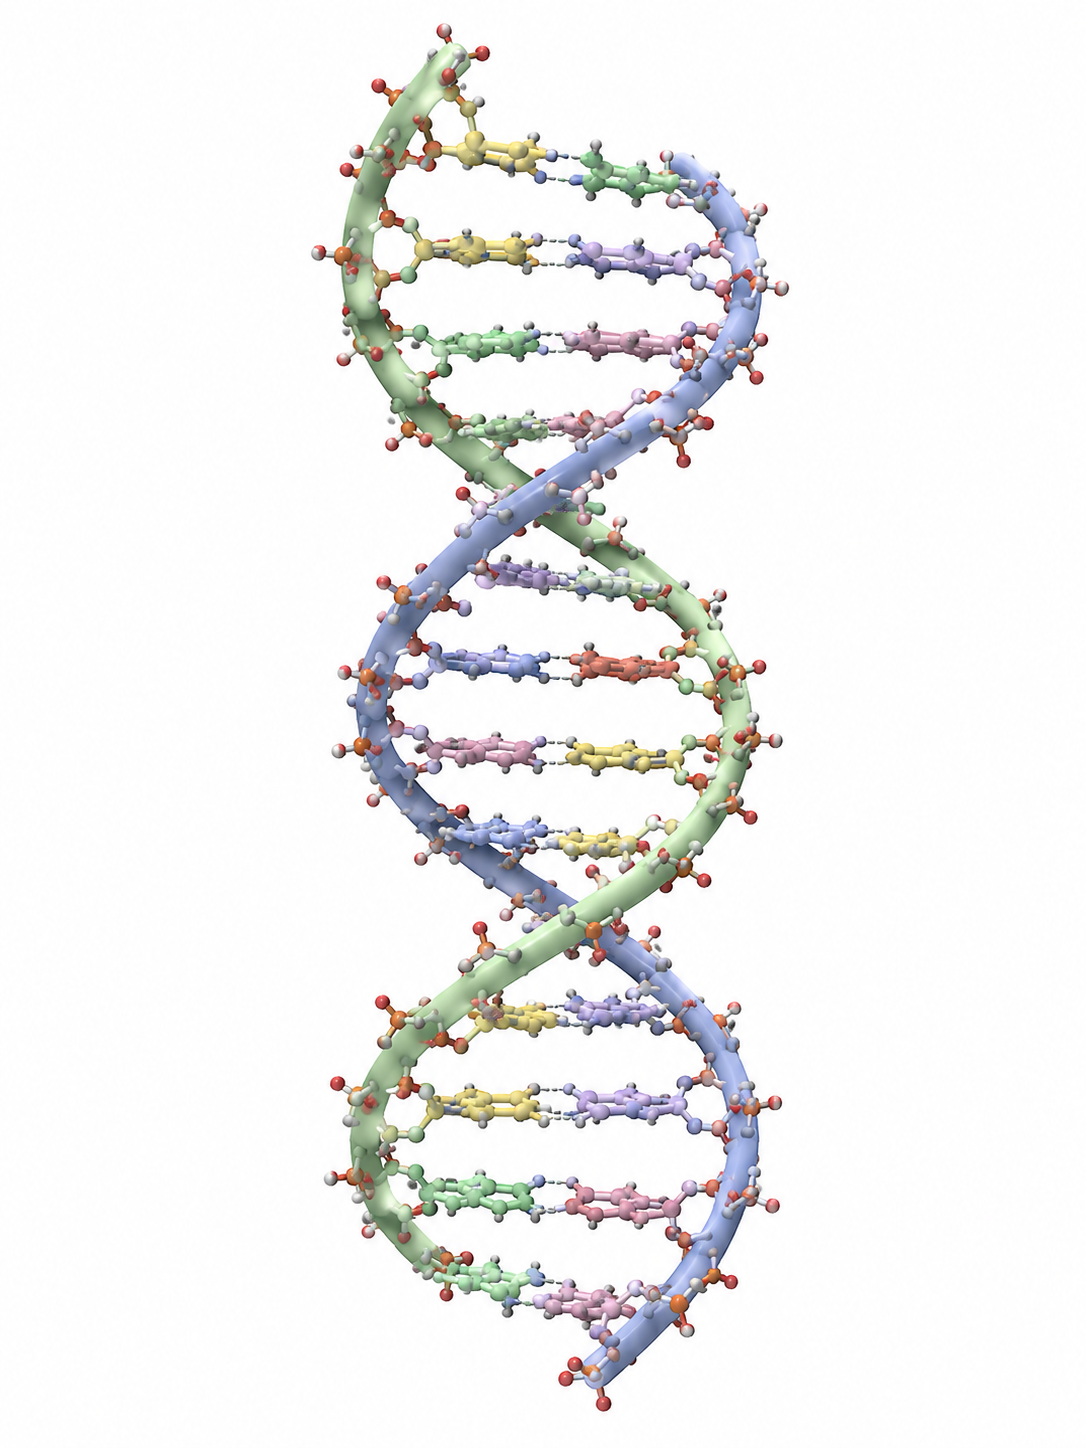
\includegraphics[width=0.9\linewidth]{images/book3/ai/fig-dna-double-helix.png}
\end{minipage}\hfill
\begin{minipage}[b]{0.62\linewidth}\centering
\begin{tikzpicture}[font=\footnotesize, line cap=round]
  % two antiparallel backbones as vertical bars, base pairs as rungs
  \draw[line width=3pt, omDef] (0,0) -- (0,5.1);
  \draw[line width=3pt, omDef!50] (2.6,0) -- (2.6,5.1);
  \foreach \i/\l/\r/\n in {0/A/T/2,1/G/C/3,2/T/A/2,3/C/G/3,4/A/T/2,5/G/C/3,6/C/G/3,7/T/A/2,8/G/C/3,9/A/T/2} {
    \pgfmathsetmacro{\y}{0.3+0.5*\i}
    \draw[thick, omExo!80!black, fill=omExo!20] (0.1,\y-0.14) rectangle (1.2,\y+0.14);
    \draw[thick, omExo!80!black, fill=omExo!20] (1.4,\y-0.14) rectangle (2.5,\y+0.14);
    \node[font=\scriptsize] at (0.65,\y) {\l}; \node[font=\scriptsize] at (1.95,\y) {\r};
    \ifnum\n=3 \draw[dashed] (1.2,\y-0.08) -- (1.4,\y-0.08) (1.2,\y) -- (1.4,\y) (1.2,\y+0.08) -- (1.4,\y+0.08);
    \else \draw[dashed] (1.2,\y-0.05) -- (1.4,\y-0.05) (1.2,\y+0.05) -- (1.4,\y+0.05); \fi
  }
  \node[anchor=south, omDef] at (0,5.15) {$5'$}; \node[anchor=north, omDef] at (0,-0.05) {$3'$};
  \node[anchor=south, omDef!70!black] at (2.6,5.15) {$3'$}; \node[anchor=north, omDef!70!black] at (2.6,-0.05) {$5'$};
  \draw[<->, thick] (3.2,0.3) -- (3.2,4.8) node[midway, right, align=left] {diez pares de bases\\ $= \qty{3.4}{nm}$\\ $=$ una vuelta};
  \draw[<->, thick] (3.2,-0.6) -- (3.2,0.3) node[midway, right] {};
  \draw[<->, thick] (0,-0.9) -- (2.6,-0.9) node[midway, below] {\qty{2}{nm}};
  \draw[<->, thick] (-0.5,0.3) -- (-0.5,0.8) node[midway, left] {\qty{0.34}{nm}};
  \node[anchor=west, align=left, font=\scriptsize] at (3.2,5.2) {2 enlaces de hidrógeno A--T\\ 3 enlaces de hidrógeno G--C};
\end{tikzpicture}
\end{minipage}

{\small A la izquierda: un modelo de la \omterm{thm:b1:nucleic-acids:helix}{doble hélice}; los dos esqueletos se
enrollan alrededor de los \omterm{thm:b1:nucleic-acids:helix}{pares de bases} apilados y dejan un surco mayor y
un surco menor. A la derecha: esos mismos diez \omterm{thm:b1:nucleic-acids:helix}{pares de bases} desenrollados
en escalera: hebras antiparalelas, pares complementarios de igual anchura,
\qty{0.34}{nm} por par y \qty{3.4}{nm} por vuelta.}
\end{omfigure}

\begin{example}[Leer una hebra]\label{ex:b1:nucleic-acids:complement}
Si una hebra dice $5'$-ATGGCATTC-$3'$, su compañera, escrita de
$5' \to 3'$, es $5'$-GAATGCCAT-$3'$: complétese cada \omterm{def:b1:nucleic-acids:nucleotide}{base} y después
inviértase el orden. Nueve pares, \qty{3.1}{nm} de hélice y veintidós
\omterm{def:b1:water-small-molecules:water}{enlaces de hidrógeno} (cinco G--C y cuatro A--T). Un cromosoma humano de
\num{2.5e8} pares mide \qty{8.5}{cm} de largo en esta forma y debe plegarse
cien mil veces para caber en un núcleo (\cref{ch:b1:genomes}).
\end{example}

\begin{proposition}[Qué mantiene unida la hélice]\label{prop:b1:nucleic-acids:stability}
Los \omterm{def:b1:water-small-molecules:water}{enlaces de hidrógeno} entre las \omterm{def:b1:nucleic-acids:nucleotide}{bases} apareadas dan la especificidad; el
\emph{apilamiento}\index{apilamiento de bases} de las \omterm{def:b1:nucleic-acids:nucleotide}{bases} planas unas
sobre otras --- contactos de \omterm{def:b1:water-small-molecules:bonds}{van der Waals} y el \omterm{prop:b1:water-small-molecules:properties}{efecto hidrófobo}, que
mantiene las \omterm{def:b1:nucleic-acids:nucleotide}{bases} fuera del agua --- aporta la mayor parte de la
estabilidad; los esqueletos, cargados negativamente, se repelen, y la hélice
solo es estable en presencia de cationes (el $\mathrm{Mg^{2+}}$ y el
$\mathrm{Na^+}$ fisiológicos, o las proteínas básicas de la cromatina) que
apantallen la carga. Un par G--C, con tres \omterm{def:b1:water-small-molecules:water}{enlaces de hidrógeno} y un
\omterm{prop:b1:nucleic-acids:stability}{apilamiento} más fuerte, aguanta mejor que un par A--T.
\end{proposition}

\section{Fusión e hibridación}

\begin{definition}[Desnaturalización, temperatura de fusión]\label{def:b1:nucleic-acids:melting}
El calor, o un pH extremo, separa las dos hebras del \omterm{def:b1:nucleic-acids:chain}{ADN}: es la
\emph{desnaturalización}\index{desnaturalización (ADN)} (fusión), una
transición cooperativa que ocurre en unos pocos grados y cuyo punto medio es
la \emph{temperatura de fusión}\index{temperatura de fusión} $T_m$. Va
acompañada del \emph{efecto hipercrómico}: las hebras sencillas absorben
alrededor de un \qty{40}{\%} más de luz ultravioleta a \qty{260}{nm} que
esas mismas \omterm{def:b1:nucleic-acids:nucleotide}{bases} apiladas en una hélice. $T_m$ sube con el contenido en
$G + C$ (\qty{0.4}{\celsius} por punto porcentual), con la concentración
salina y con la longitud; en una sal \qty{0.15}{mol/L}, un \omterm{def:b1:nucleic-acids:chain}{ADN} largo con un
\qty{50}{\%} de $G + C$ funde cerca de \qty{90}{\celsius}. Al enfriarse
despacio, las hebras encuentran a sus complementarias y rehacen la hélice:
es la \emph{renaturalización}, o \emph{hibridación}\index{hibridación}
cuando las hebras proceden de fuentes distintas.
\end{definition}

\begin{omfigure}
\begin{tikzpicture}
\begin{axis}[
  width=0.86\linewidth, height=6.0cm,
  axis x line=bottom, axis y line=left,
  xmin=60, xmax=105, ymin=0.95, ymax=1.5,
  xlabel={temperatura (\unit{\celsius})}, ylabel={absorbancia relativa a \qty{260}{nm}},
  xlabel style={font=\small, at={(axis description cs:0.5,-0.12)}, anchor=north},
  ylabel style={font=\small},
  tick label style={font=\small}, xtick={60,70,80,90,100}, ytick={1.0,1.2,1.4},
  legend style={font=\small, at={(0.03,0.97)}, anchor=north west, draw=none},
  clip=false,
]
\addplot[very thick, omDef, domain=60:105, samples=120] {1+0.4/(1+exp(-(x-77)/1.5))};
\addlegendentry{\qty{30}{\%} de $G+C$: $T_m = \qty{77}{\celsius}$}
\addplot[very thick, omThm, domain=60:105, samples=120] {1+0.4/(1+exp(-(x-93)/1.5))};
\addlegendentry{\qty{70}{\%} de $G+C$: $T_m = \qty{93}{\celsius}$}
\draw[dashed, gray] (axis cs:60,1.2) -- (axis cs:93,1.2);
\draw[dashed, gray] (axis cs:77,0.95) -- (axis cs:77,1.2);
\draw[dashed, gray] (axis cs:93,0.95) -- (axis cs:93,1.2);
\end{axis}
\end{tikzpicture}

{\small Curvas de fusión de dos \omterm{def:b1:nucleic-acids:chain}{ADN} en la misma sal. La absorbancia sube un
\qty{40}{\%} a medida que se separan las hebras, en unos pocos grados; el
punto medio, $T_m$, es mayor para el \omterm{def:b1:nucleic-acids:chain}{ADN} más rico en pares G--C.}
\end{omfigure}

\begin{method}[Medida de ácidos nucleicos por absorbancia]\label{met:b1:nucleic-acids:absorbance}
\begin{enumerate}
  \item Las \omterm{def:b1:nucleic-acids:nucleotide}{bases} absorben luz ultravioleta con un máximo a \qty{260}{nm}.
        En una cubeta de \qty{1}{cm}, una absorbancia de $1.0$ corresponde a
        \qty{50}{\micro g/mL} de \omterm{def:b1:nucleic-acids:chain}{ADN} bicatenario (\qty{40}{\micro g/mL} de
        \omterm{def:b1:nucleic-acids:chain}{ARN}, \qty{33}{\micro g/mL} de \omterm{def:b1:nucleic-acids:chain}{ADN} monocatenario).
  \item El cociente $A_{260}/A_{280}$ es de $1.8$ para el \omterm{def:b1:nucleic-acids:chain}{ADN} puro y de
        $2.0$ para el \omterm{def:b1:nucleic-acids:chain}{ARN} puro; las proteínas absorben a \qty{280}{nm} y lo
        rebajan.
  \item Para seguir la fusión, regístrese $A_{260}$ mientras se calienta
        despacio; el punto medio de la curva es $T_m$ y su pendiente, una
        medida de la homogeneidad de la muestra.
  \item Para detectar una secuencia, desnaturalícese la muestra y añádase
        una hebra sencilla marcada complementaria de ella (una
        \emph{sonda}); hibrida solo donde está su complementaria, y la
        marca señala el lugar: en un gel, en un cromosoma, en un \omterm{def:b1:body-plans-tissues:tissue}{tejido}.
\end{enumerate}
\end{method}

\begin{omfigure}
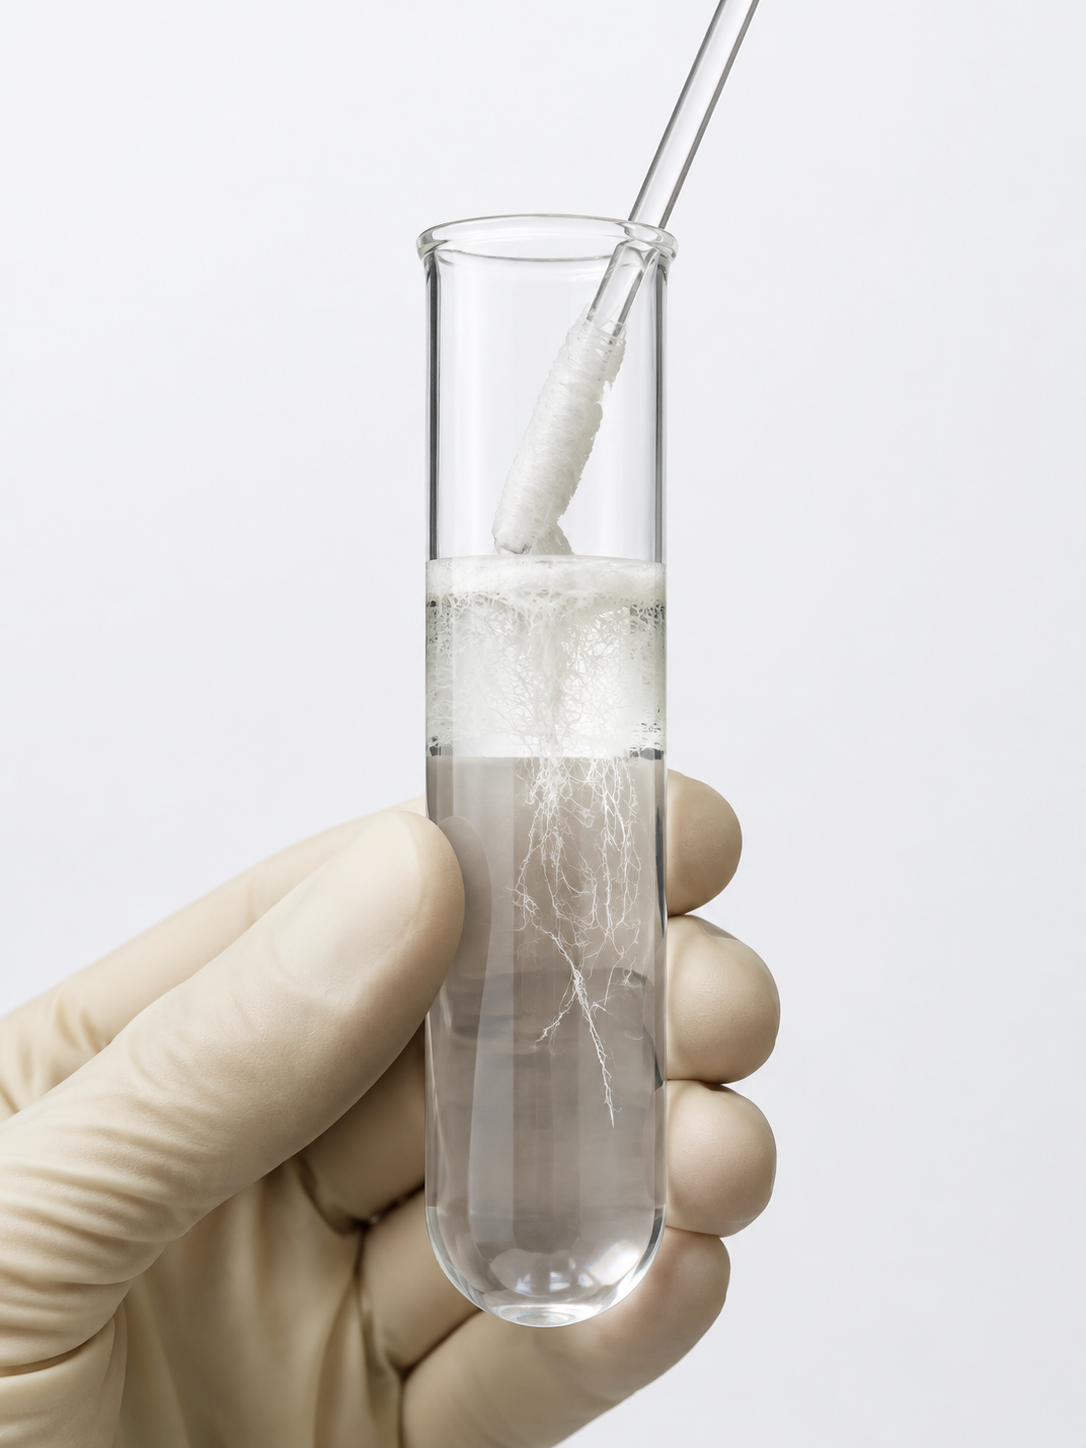
\includegraphics[width=0.3\linewidth]{images/book3/ai/b3-11-dna-precipitate.png}

{\small \omterm{def:b1:nucleic-acids:chain}{ADN} precipitado con etanol frío a partir de un lisado celular y
enrollado en una varilla de vidrio: unos pocos miligramos de la molécula,
visibles como fibras porque cada una tiene millones de \omterm{thm:b1:nucleic-acids:helix}{pares de bases}.}
\end{omfigure}

\begin{example}[Una sonda encuentra un gen]\label{ex:b1:nucleic-acids:probe}
Una sonda de veinte \omterm{def:b1:nucleic-acids:nucleotide}{nucleótidos} complementaria de un gen, a
\qty{5}{\celsius} por debajo de su propia $T_m$, se une a su complementaria
exacta y a nada más en tres mil millones de \omterm{thm:b1:nucleic-acids:helix}{pares de bases}: un solo
desapareamiento entre veinte baja la $T_m$ varios grados y el híbrido
desapareado funde. La especificidad del apareamiento de \omterm{def:b1:nucleic-acids:nucleotide}{bases}, multiplicada
por veinte posiciones, es aquello en lo que se apoya toda prueba de \omterm{def:b1:nucleic-acids:chain}{ADN},
desde la paternidad hasta la detección de patógenos.
\end{example}

\section{El ARN}

\begin{definition}[Los ARN]\label{def:b1:nucleic-acids:rnas}
El \omterm{def:b1:nucleic-acids:chain}{ARN} suele ser monocatenario y se pliega sobre sí mismo allí donde lo
permiten tramos complementarios cortos, formando horquillas, bucles y
protuberancias --- una \emph{estructura secundaria} --- que luego se
compacta en una forma. Tres clases sostienen el flujo de la información
genética (\cref{ch:b1:gene-expression}): el \emph{ARN
mensajero}\index{ARN mensajero} (ARNm), una copia de un gen que lee el
ribosoma; el \emph{ARN de transferencia}\index{ARN de transferencia}
(ARNt), unos \qty{75}{} \omterm{def:b1:nucleic-acids:nucleotide}{nucleótidos} plegados en trébol, que lleva un
aminoácido en su extremo $3'$ y un \emph{anticodón} que se aparea con el
mensaje; y el \emph{ARN ribosómico}\index{ARN ribosómico} (ARNr), el núcleo
estructural y catalítico del ribosoma, cuatro quintas partes del \omterm{def:b1:nucleic-acids:chain}{ARN} de una
\omterm{def:b1:cell-unit-of-life:cell}{célula}. Muchos otros \omterm{def:b1:nucleic-acids:chain}{ARN} regulan, cortan y guían (volumen del tercer año).
\end{definition}

\begin{omfigure}
\begin{tikzpicture}[font=\footnotesize, line cap=round, >=Stealth]
  % acceptor stem (vertical, top)
  \draw[line width=2.5pt, omDef] (0,0) -- (0,2.2);
  \draw[line width=2.5pt, omDef] (0.5,0) -- (0.5,2.2);
  \foreach \y in {0.3,0.65,1.0,1.35,1.7} { \draw[thick, omExo!80!black] (0,\y) -- (0.5,\y); }
  \node[anchor=south] at (0,2.25) {$5'$};
  \draw[line width=2.5pt, omDef] (0.5,2.2) -- (0.5,2.9) -- (1.0,3.2);
  \node[anchor=west] at (1.0,3.2) {$3'$-CCA: aquí se une el aminoácido};
  % D arm (left)
  \draw[line width=2.5pt, omDef] (0,0) -- (-1.4,0) (0,-0.5) -- (-1.4,-0.5);
  \foreach \x in {-0.3,-0.65,-1.0} { \draw[thick, omExo!80!black] (\x,0) -- (\x,-0.5); }
  \draw[line width=2.5pt, omDef] (-1.4,0) arc (90:270:0.25);
  \node[anchor=east, align=right] at (-1.8,-0.25) {brazo D};
  % T arm (right)
  \draw[line width=2.5pt, omDef] (0.5,0) -- (1.9,0) (0.5,-0.5) -- (1.9,-0.5);
  \foreach \x in {0.8,1.15,1.5} { \draw[thick, omExo!80!black] (\x,0) -- (\x,-0.5); }
  \draw[line width=2.5pt, omDef] (1.9,0) arc (90:-90:0.25);
  \node[anchor=west, align=left] at (2.3,-0.25) {brazo T};
  % anticodon stem (down)
  \draw[line width=2.5pt, omDef] (0,-0.5) -- (0,-2.2) (0.5,-0.5) -- (0.5,-2.2);
  \foreach \y in {-0.85,-1.2,-1.55,-1.9} { \draw[thick, omExo!80!black] (0,\y) -- (0.5,\y); }
  \draw[line width=2.5pt, omDef] (0,-2.2) arc (180:360:0.25);
  \foreach \x in {0.1,0.25,0.4} { \fill[omThm] (\x,-2.5) circle (0.06); }
  \node[anchor=north, align=center] at (0.25,-2.65) {bucle del anticodón: tres bases\\ que se aparean con un codón del ARNm};
  \node[anchor=west, align=left, gray] at (2.3,1.2) {cuatro brazos de bases apareadas\\ (el trébol), plegados en tres\\ dimensiones en forma de L};
\end{tikzpicture}

{\small Un \omterm{def:b1:nucleic-acids:rnas}{ARN de transferencia} en su estructura secundaria en trébol: una
sola hebra de unos 75 \omterm{def:b1:nucleic-acids:nucleotide}{nucleótidos} apareada consigo misma en cuatro brazos.
El aminoácido se transporta en el extremo $3'$; el anticodón, en el extremo
opuesto, lee el mensaje.}
\end{omfigure}

\begin{remark}[El ARN puede ser catalizador]\label{rem:b1:nucleic-acids:ribozyme}
Algunos \omterm{def:b1:nucleic-acids:chain}{ARN} son enzimas (\emph{ribozimas}): el enlace peptídico de todas las
proteínas lo forma el \omterm{def:b1:nucleic-acids:rnas}{ARN ribosómico}, y no una proteína, y algunos \omterm{def:b1:nucleic-acids:chain}{ARN} se
cortan y se empalman a sí mismos. Una molécula que a la vez lleva
información y cataliza reacciones es de lo que pudo estar hecho un primer
sistema vivo; el mundo del \omterm{def:b1:nucleic-acids:chain}{ADN} y las proteínas sería entonces una división
del trabajo posterior, con el \omterm{def:b1:nucleic-acids:chain}{ARN} conservado en su centro.
\end{remark}

\section{Ejercicios}

\begin{exercise}[$\star$]\label{exo:b1:nucleic-acids:1}
Nómbrense las tres partes de un \omterm{def:b1:nucleic-acids:nucleotide}{nucleótido} y las dos diferencias entre un
ribonucleótido y un desoxirribonucleótido.
\end{exercise}

\begin{exercise}[$\star$]\label{exo:b1:nucleic-acids:2}
Escríbase la hebra complementaria de $5'$-GGATCCTA-$3'$ en el sentido
$5' \to 3'$ y cuéntense sus \omterm{def:b1:water-small-molecules:water}{enlaces de hidrógeno}.
\end{exercise}

\begin{exercise}[$\star$]\label{exo:b1:nucleic-acids:3}
Un \omterm{def:b1:nucleic-acids:chain}{ADN} contiene un \qty{22}{\%} de adenina. Dense los porcentajes de T, G y
C, y el contenido en $G + C$.
\end{exercise}

\begin{exercise}[$\star$]\label{exo:b1:nucleic-acids:4}
A partir de la figura de la fusión, ¿cuál es la $T_m$ de un \omterm{def:b1:nucleic-acids:chain}{ADN} con un
\qty{50}{\%} de $G + C$ en las mismas condiciones, y cuánto sube la
absorbancia al fundirse?
\end{exercise}

\begin{exercise}[$\star\star$]\label{exo:b1:nucleic-acids:5}
Calcúlense la longitud del cromosoma de \emph{E. coli} ($\num{4.6e6}$ \omterm{thm:b1:nucleic-acids:helix}{pares
de bases}) en milímetros, su número de vueltas y el factor de compactación
necesario para que quepa en una \omterm{def:b1:cell-unit-of-life:cell}{célula} de \qty{2}{\micro m}.
\end{exercise}

\begin{exercise}[$\star\star$]\label{exo:b1:nucleic-acids:6}
Explíquese por qué las dos hebras del \omterm{def:b1:nucleic-acids:chain}{ADN} deben ser antiparalelas, usando la
geometría del esqueleto de azúcar y fosfato y la exigencia de que todos los
\omterm{thm:b1:nucleic-acids:helix}{pares de bases} tengan la misma anchura.
\end{exercise}

\begin{exercise}[$\star\star$]\label{exo:b1:nucleic-acids:7}
Una disolución de \omterm{def:b1:nucleic-acids:chain}{ADN} tiene $A_{260} = 0.35$ en una cubeta de \qty{1}{cm} y
$A_{280} = 0.20$. Calcúlese la concentración y coméntese la pureza.
¿Cuántos \omterm{thm:b1:nucleic-acids:helix}{pares de bases} hay en \qty{1}{mL}, si la masa media de un par es de
\qty{650}{Da}?
\end{exercise}

\begin{exercise}[$\star\star$]\label{exo:b1:nucleic-acids:8}
Explíquense el efecto hipercrómico y por qué la curva de fusión de un \omterm{def:b1:nucleic-acids:chain}{ADN}
puro es abrupta mientras que la de una mezcla de \omterm{def:b1:nucleic-acids:chain}{ADN} de muchas especies está
extendida.
\end{exercise}

\begin{exercise}[$\star\star$]\label{exo:b1:nucleic-acids:9}
Una sonda de veinte \omterm{def:b1:nucleic-acids:nucleotide}{nucleótidos} tiene $T_m = \qty{62}{\celsius}$ con su
complementaria exacta; un desapareamiento baja la $T_m$ unos
\qty{5}{\celsius}. ¿A qué temperatura debería hacerse la \omterm{def:b1:nucleic-acids:melting}{hibridación} para
detectar la secuencia exacta y rechazar los desapareamientos sencillos? ¿Qué
ocurre a \qty{45}{\celsius}?
\end{exercise}

\begin{exercise}[$\star\star\star$]\label{exo:b1:nucleic-acids:10}
Las reglas de \omterm{prop:b1:nucleic-acids:chargaff}{Chargaff} se cumplen en el \omterm{def:b1:nucleic-acids:chain}{ADN} bicatenario, pero no en el \omterm{def:b1:nucleic-acids:chain}{ARN}
ni en el \omterm{def:b1:nucleic-acids:chain}{ADN} de ciertos virus pequeños. Explíquese qué dice cada excepción
sobre la estructura de esos ácidos nucleicos.
\end{exercise}

\begin{exercise}[$\star\star\star$]\label{exo:b1:nucleic-acids:11}
Dos \omterm{def:b1:water-small-molecules:water}{enlaces de hidrógeno} mantienen un par A--T, y sin embargo una hélice de
mil pares A--T es estable a \qty{60}{\celsius}, mientras que un par aislado
ni siquiera se forma. Explíquese con las ideas del
\cref{ch:b1:water-small-molecules} (enlaces débiles, cooperatividad,
\omterm{prop:b1:nucleic-acids:stability}{apilamiento}), y dígase qué implica esto para la fidelidad de una sonda.
\end{exercise}

\begin{exercise}[$\star\star\star$]\label{exo:b1:nucleic-acids:12}
``La estructura del \omterm{def:b1:nucleic-acids:chain}{ADN} es la explicación de la herencia.'' Discútase en un
párrafo: qué explica de inmediato la \omterm{thm:b1:nucleic-acids:helix}{doble hélice} (la copia, la mutación
como cambio de secuencia), qué no explica por sí sola (cómo la secuencia
llega a ser una proteína) y por qué el modelo de Watson y Crick se aceptó
antes de cualquier prueba bioquímica.
\end{exercise}

\section{Problema: el genoma de un virus}

\begin{problem}[{Problema de fin de semana --- el ADN del fago $\lambda$
medido, pesado, contado, fundido y empaquetado en su cápside, hasta llegar a
su temperatura de fusión y a su longitud de contorno}]
\label{pb:b1:nucleic-acids:1}
El genoma del bacteriófago $\lambda$ es un único \omterm{def:b1:nucleic-acids:chain}{ADN} bicatenario lineal de
\num{48502} \omterm{thm:b1:nucleic-acids:helix}{pares de bases} con un contenido en $G + C$ del \qty{49.9}{\%}.
Está empaquetado en una cápside icosaédrica de \qty{55}{nm} de diámetro
interno. Tómense \qty{0.34}{nm} por \omterm{thm:b1:nucleic-acids:helix}{par de bases}, \qty{2.0}{nm} de diámetro
de hélice, \qty{650}{Da} por \omterm{thm:b1:nucleic-acids:helix}{par de bases} y $T_m = 81.5 + 16.6\log_{10}[\mathrm{Na^+}]
+ 0.41\,(\%\,G{+}C) - 500/L$ en grados Celsius, con $[\mathrm{Na^+}]$ en
\unit{mol/L} y $L$ la longitud en \omterm{thm:b1:nucleic-acids:helix}{pares de bases}.

\medskip
\noindent\textbf{Parte I --- Medido y pesado.}
\begin{enumerate}
  \item Calcúlese la longitud de contorno de la molécula en micrómetros.
  \item Calcúlese el número de vueltas de la hélice.
  \item Calcúlese su masa molar en dalton.
  \item Calcúlese la masa de una molécula en gramos.
  \item Calcúlense el número de grupos fosfato y, con ello, la carga neta
        de la molécula.
  \item Calcúlese el número de \omterm{def:b1:nucleic-acids:nucleotide}{nucleótidos} de cada \omterm{def:b1:nucleic-acids:nucleotide}{base} (A, T, G, C).
  \item Calcúlese el número total de \omterm{def:b1:water-small-molecules:water}{enlaces de hidrógeno} que mantienen
        unidas las dos hebras.
\end{enumerate}

\medskip
\noindent\textbf{Parte II --- Fundido.}
\begin{enumerate}[resume]
  \item Calcúlese $T_m$ en sodio \qty{0.1}{mol/L}.
  \item Calcúlese $T_m$ en sodio \qty{0.01}{mol/L} y explíquese por qué la
        sal estabiliza la hélice.
  \item El genoma de $\lambda$ contiene una región de \qty{1000}{} pares
        con un \qty{35}{\%} de $G + C$ y otra con un \qty{62}{\%}.
        Calcúlese la $T_m$ de cada región en sodio \qty{0.1}{mol/L} y
        descríbase la forma de la curva de fusión de la molécula entera.
  \item Una disolución de \omterm{def:b1:nucleic-acids:chain}{ADN} de $\lambda$ tiene $A_{260} = 0.50$ antes de
        la fusión. ¿Cuál es su concentración, y cuánto valdrá $A_{260}$
        tras la fusión completa?
  \item ¿Cuántas moléculas de $\lambda$ hay en \qty{1}{mL} de esa
        disolución?
  \item Los dos extremos del genoma de $\lambda$ son salientes
        monocatenarios de 12 \omterm{def:b1:nucleic-acids:nucleotide}{nucleótidos}, complementarios entre sí, por los
        que la molécula se circulariza en el hospedador. Calcúlese su
        $T_m$ (úsese $L = 12$) y dígase por qué, pese a ello, el círculo
        aguanta a \qty{37}{\celsius} dentro de la \omterm{def:b1:cell-unit-of-life:cell}{célula}.
\end{enumerate}

\medskip
\noindent\textbf{Parte III --- Empaquetado.}
\begin{enumerate}[resume]
  \item Calcúlese el volumen del \omterm{def:b1:nucleic-acids:chain}{ADN} como cilindro.
  \item Calcúlese el volumen interno de la cápside.
  \item ¿Qué fracción de la cápside ocupa el \omterm{def:b1:nucleic-acids:chain}{ADN}? Compárese con el
        empaquetamiento más denso de cilindros paralelos (\qty{91}{\%}).
  \item El \omterm{def:b1:nucleic-acids:chain}{ADN} lleva \num{97000} cargas negativas dentro de una esfera de
        \qty{55}{nm}. Explíquese qué debe acompañar al \omterm{def:b1:nucleic-acids:chain}{ADN} dentro de la
        cápside, y por qué el \omterm{def:b1:nucleic-acids:chain}{ADN} empaquetado ejerce sobre la envoltura
        una presión (de decenas de atmósferas) que ayuda a inyectarlo en
        una bacteria.
  \item La molécula debe doblarse en bucles de radio comparable al de la
        cápside. El \omterm{def:b1:nucleic-acids:chain}{ADN} se resiste a doblarse por debajo de un radio de
        unos \qty{50}{nm}. Coméntese.
\end{enumerate}

\medskip
\noindent\textbf{Parte IV --- Leído.}
\begin{enumerate}[resume]
  \item Una hebra del genoma empieza por $5'$-GGGCGGCGACCT-$3'$. Escríbase
        la hebra complementaria de $5' \to 3'$.
  \item Si un gen de \num{1200} \omterm{thm:b1:nucleic-acids:helix}{pares de bases} se transcribe a un ARNm,
        ¿cuál es la longitud del ARNm en \omterm{def:b1:nucleic-acids:nucleotide}{nucleótidos} y, a \qty{330}{Da} por
        \omterm{def:b1:nucleic-acids:nucleotide}{nucleótido}, su masa?
  \item El genoma tiene \qty{75}{} genes en \num{48502} pares. ¿Qué
        fracción del genoma es codificante si el gen medio tiene \num{600}
        pares? Compárese con el genoma humano (\qty{1.5}{\%}).
  \item El genoma se replica en \qty{20}{min} a \qty{37}{\celsius} con las
        enzimas del hospedador. Calcúlese la velocidad en \omterm{thm:b1:nucleic-acids:helix}{pares de bases}
        por segundo si la replicación empieza en un origen y avanza en
        ambos sentidos.
  \item ¿Cuántos \omterm{def:b1:water-small-molecules:water}{enlaces de hidrógeno} se rompen por segundo en las dos
        horquillas durante la replicación (úsese la media por par de la
        pregunta 7)?
  \item Una mutación cambia un par G--C por uno A--T. ¿Cuánto varía la
        $T_m$ de la molécula entera? ¿Podría detectarlo la fusión?
  \item Enúnciese el resultado: la \omterm{def:b1:nucleic-acids:melting}{temperatura de fusión} del \omterm{def:b1:nucleic-acids:chain}{ADN} de
        $\lambda$ en sodio \qty{0.1}{mol/L} y su longitud de contorno, y la
        compactación con la que cabe en la cápside.
\end{enumerate}
\end{problem}
